\section{Agricultural Robots}

	Agricultural robots are designed to be implemented on an unstructured environment. Hence, these robots are expected to be dynamic, uncertain, complex, highly variable, and hostile. In order to build an agricultural robot, multiple design principles are taken into consideration. This includes product specification such as speed, system analysis such as the function, concept development such as alternative methods, feasibility, and what not. Figure~\ref{fig:robot} shows the flowchart  of the implementation of concepts on an agricultural robot.~\cite{Edan}

\begin{figure}[!b]
	\centering
		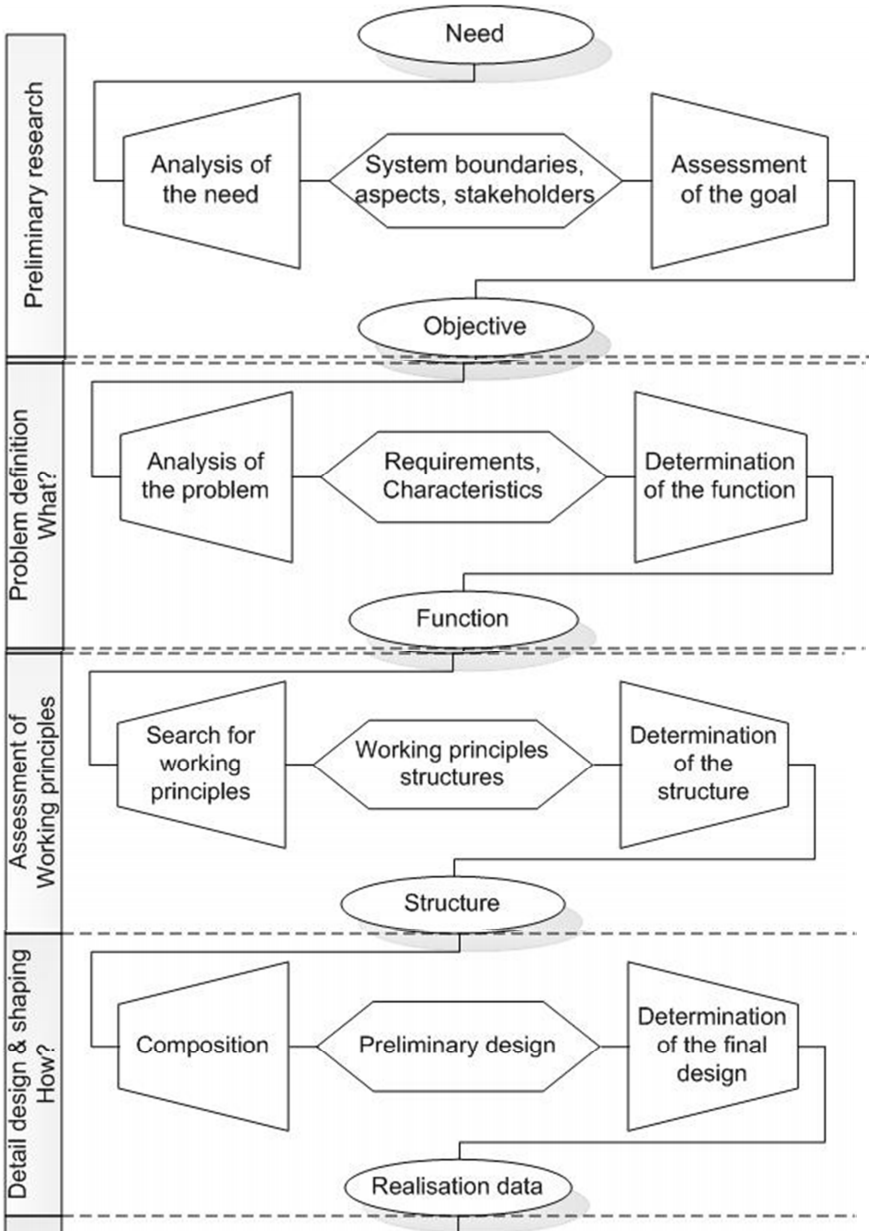
\includegraphics[width=2.5 in]{robot}
	\caption{Flowchart of Agricultural Robot Design}
	\label{fig:robot}
\end{figure}

\section{Raspberry Pi 3 Model B}

	Raspberry Pi is a low-cost microcomputer originally designed to aide young people in programming. It is advantageous in terms of size, portability, cost, programmability, and connectivity.~\cite{vid} Raspberry Pi is mounted on a credit card-sized board and has multiple feature ports such as USB 2.0, HDMI, Power, SD Card, and many more depending on the model.

	On this research, Raspberry Pi 3 model B is used. Its features include:
\begin{itemize}
\item {A 1.2GHz 64-bit quad-core ARMv8 CPU}
\item {802.11n Wireless LAN}
\item {Bluetooth 4.1}
\item {Bluetooth Low Energy (BLE)]
\item {1GB RAM}
\item {4 USB ports}
\item {40 GPIO pins}
\item {Full HDMI port}
\item {Ethernet port}
\item {Combined 3.5mm audio jack and composite video}
\item {Camera interface (CSI)}
\item {Display interface (DSI)}
\item {Micro SD card slot (now push-pull rather than push-push)}
\item {VideoCore IV 3D graphics core}
\end{itemize}

Figures~\ref{fig:display},~\ref{fig:camera},~\ref{fig:gpioexpansion},~\ref{fig:powerin} and~\ref{fig:run} show the schematic diagrams essential to this research.

\begin{figure}[!htbp]
	\centering
		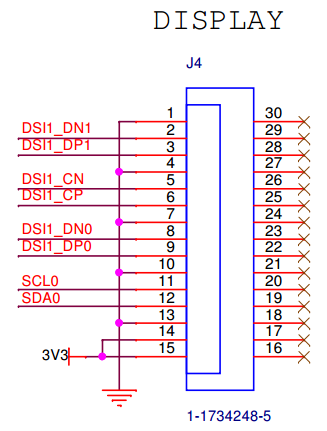
\includegraphics[width=2.5 in]{display}
	\caption{Schematic of Display}
	\label{fig:display}
\end{figure}

\begin{figure}[!htbp]
	\centering
		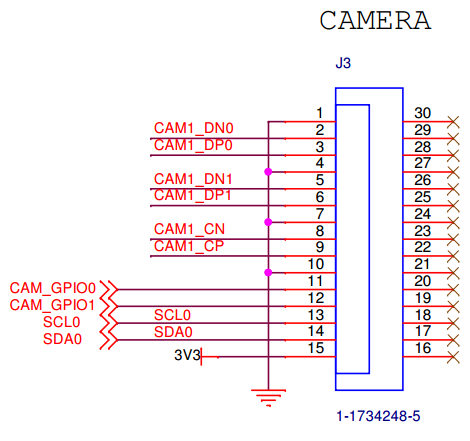
\includegraphics[width=2.5 in]{camera}
	\caption{Schematic of Camera Port}
	\label{fig:camera}
\end{figure}

\begin{figure}[!htbp]
	\centering
		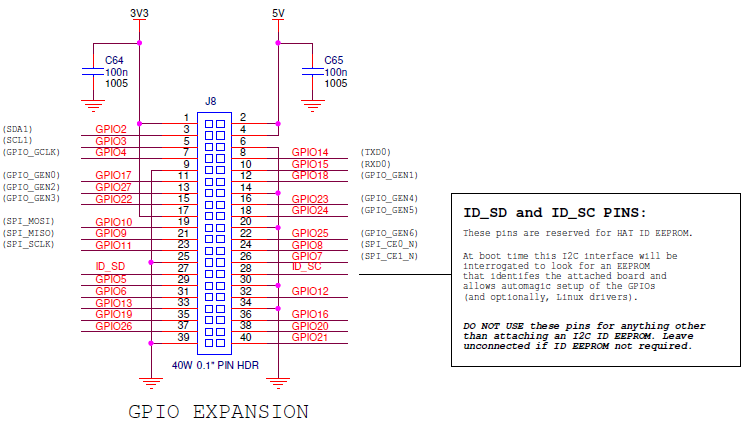
\includegraphics[width=2.5 in]{gpioexpansion}
	\caption{Schematic of GPIO Expansion}
	\label{fig:gpioexpansion}
\end{figure}

\begin{figure}[!htbp]
	\centering
		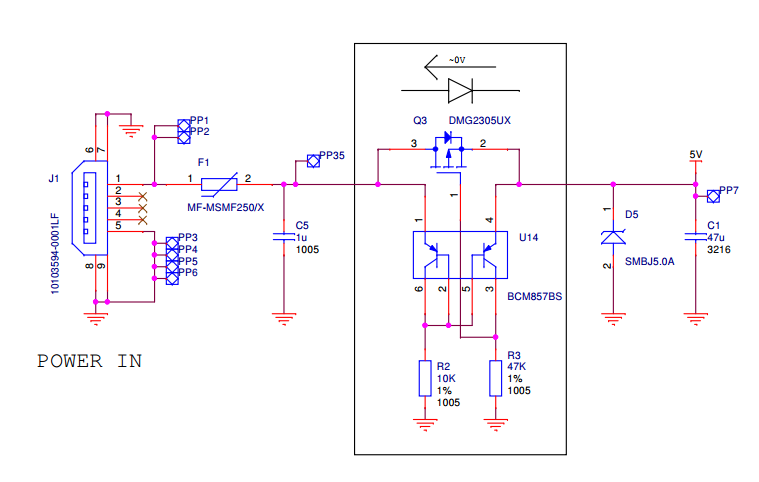
\includegraphics[width=2.5 in]{powerin}
	\caption{Schematic of Power Input}
	\label{fig:powerin}
\end{figure}

\begin{figure}[!htbp]
	\centering
		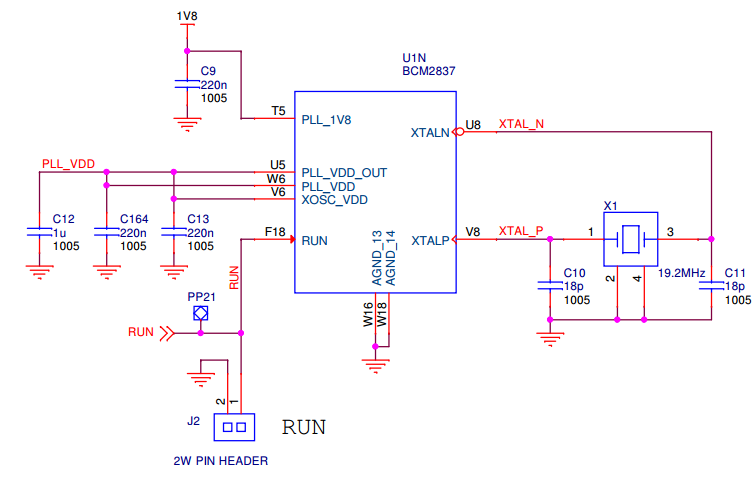
\includegraphics[width=2.5 in]{run}
	\caption{Schematic of RUN}
	\label{fig:run}
\end{figure}

\section{Raspberry Pi Camera Module}

The PiCamera is a camera module for Raspberry Pi that allows the users to capture still photos and record videos in high definition. A camera port on the microcomputer is available for this device. In this port, the camera is connected while Pi is still switched off and once it is connected to the board, the devices are switched on. The camera software is available on the Raspberry Pi Configuration Tool. Python3 is utilized in order to preview the camera. Figure~\ref{fig:code} shows the code to be executed in order to allow the preview of the camera.~\cite{camers}

\begin{figure}[!htbp]
	\centering
		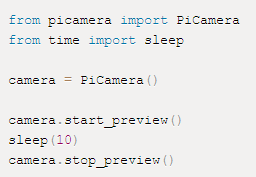
\includegraphics[]{code}
	\caption{Code for Camera  Preview}
	\label{fig:code}
\end{figure}

\section{Virtual Network Computing}
Virtual Network Computing (VNC) is a graphical sharing system on a desktop that allows remote access and control of a desktop interface of on device from another. The events from the controller such as keyboard and mouse are transmitted to the screen over the network from the remote host. 
	On the Raspberry Pi, it is necessary to install the TightVNC package in order to utilize this system. To install this package, the code  \textsl{sudo apt-get install tightvncserver} is used. Running the TightVNC Server would prompt the user to input the password \textsl{tightvncserver}. From the terminal, VNC is started. A session on VNC display one with full HD resolution is written as \textsl{vncserver :1 -geometry 1920x1080 -depth 24}.
	In order to run the VNC server on the Pi, a command on a file is necessary. The shell script \textsl{#!/bin/sh (next line) vncserver :1 -geometry 1920x1080 -depth 24 -dpi 96} is to be created. By inputting the code \textsl{chmod +x vnc.sh}, the shell script with filename vnc.sh is made executable. In order to run the file at any time, the code \textsl{./vnc.sh} is executed.
	The procedure mentioned above is the initialization of VNC on the Pi module. With this, a VNC client on the personal computer is needed in order to connect the computer to the VNC server and have control of it.~\cite{vnc}
	
\section{IP Address}
	Internet Protocol (IP) Address is an address that is used to identify a unique device over an IP network. It is a core in network design as it is a Network Foundation service. It provides the foundation of other network and user services and it allows the interaction of devices within the network.~\cite{cisco}
	Raspberry Pi 3 model B is connected to a Local Area Network. Hence, as any device connected to a LAN, Pi is assigned a unique IP address. IP address is vital information in connecting the Pi to another machine using VNC. The code \textsl{hostname –I} reveals the IP Address of the Pi using the terminal.
		



